\subsection{Problem 3}
\subsubsection{Dynamic interaction model}

"Competition" refers to the struggle for existence between two or more individuals within or between species, whose demands more or less exceed the supply of common resources, thus exerting adverse effects on each other among these competing individuals. In this question, different types of fungi compete for space and resources to survive in the same environment, so the interaction between them is usually manifested as competition, that is, competition between different populations.Our model needs to address what types of community evolution occur between different types of fungi under the same initial environment.
\begin{itemize}
    \item [(1)] 
    \textbf{Logistic model and Lotka-Volterra model}
\end{itemize}

At the beginning, the two or more fungal populations do not compete with each other under the condition of adequate nutrient supply. However, when the number of fungi more suitable for the environment is much larger than that of the weaker species, the weaker species will lack nutrients and may die. That is, when different types of fungi compete for the same food source and space, the common outcome is that the less competitive ones go extinct and the more competitive ones reach the maximum capacity that the environment allows. The population competition model can be used to describe the process of competition between different types of fungi and to analyze the conditions that produce the evolutionary outcomes of various communities.

When fungus 1 and fungus 2 are present, an increase in the number of one inhibits the growth of the other, given limited space and resources. Several parameters are used to represent the rules\upcite{jiang2} that the two fungi obey in the process of competition as follows:
\begin{equation}\label{3.1}
    \left\{
    \begin{array}{l}
        \frac{dN_{1}}{dt}=r_{1}N_{1}(1-\frac{N_{1}}{k_{1}}-\alpha \frac{N_{2}}{k_{1}}) \\
        \frac{dN_{2}}{dt}=r_{2}N_{2}(1-\frac{N_{2}}{k_{2}}-\beta \frac{N_{1}}{k_{2}}) \\
    \end{array}
    \right.
    \end{equation}

Where,

$N_{1}$ and $N_{2}$ are the size (expressed in number) of the two fungi;

$k_{1}$ and $k_{2}$ are the maximum environmental tolerance of the two fungi;

$r_{1}$ and $r_{2}$ are the growth rate of the two fungi;

$\alpha$ is the coefficient of competition of 1 to 2;

$\beta$ is the coefficient of competition of 2 to 1.

The coefficients of competition introduced here- $\alpha$ and $\beta$ represent the amount of one fungus that can be supported by the space and resources occupied by another fungus. Therefore, the inhibition relationship between fungi 1 and 2 can be reflected by the relationship between $k_{1}$ and $k_{2}$ . Through analysis, the inhibition relationship between the two fungi can be obtained as follows:

When $k_{2} > \frac{k_{1}}{\alpha}$, Fungus 2 can inhibit Fungus 1;

When $k_{2} < \frac{k_{1}}{\alpha}$, Fungus 2 can’t inhibit Fungus 1;

When $k_{1} > \frac{k_{2}}{\beta}$, Fungus 1 can inhibit Fungus 2;

When $k_{1} < \frac{k_{2}}{\beta}$, Fungus 1 can’t inhibit Fungus 2.
\begin{itemize}
    \item [(2)] 
    \textbf{Model singularity and type analysis}
\end{itemize}

In the process of competition, when both Equations in (\ref{3.1}) are zero, both Fungi 1 and Fungi 2 stop growing, and the system is relatively stable. It's easy to know that its singularity in the first quadrant is $E_{1}(0,0),E_{2}(k_{1},0),E_{3}(0,k_{2})$ and $E_{4}(k_{1}-\alpha k_{2},k_{2}-\beta k_{1})$.

\begin{itemize}
    \item [a)] 
    The linear equations corresponding to the singularity $E_{1}(0,0)$ are
    \begin{equation}\label{}
        \left\{
        \begin{array}{l}
            \frac{dN_{1}}{dt}=r_{1}N_{1} \\
            \frac{dN_{2}}{dt}=r_{2}N_{2} \\
        \end{array}
        \right.
        \end{equation}
    
    The coefficient matrix characteristic equation of the linear equations is $(\lambda-r_{1})(\lambda-r_{2})=0$, so $E_{1}(0,0)$ is the unstable point.

    \item [b)]
    Transform the singularity $E_{2}(k_{1},0)$ as follows:
    \begin{equation}\label{}
        \widetilde{N_{1}}=N_{1}-k_{1},\widetilde{N_{2}}=N_{2}
    \end{equation}

    The corresponding linear system of equations are:
    \begin{equation}\label{}
        \left\{
        \begin{array}{l}
            \frac{d\widetilde{N_{1}}}{dt}=r_{1}(\widetilde{N_{1}}+k_{1})(\frac{-\alpha\widetilde{N_{2}}-\widetilde{N_{1}}}{k_{1}}) \\
            \frac{d\widetilde{N_{2}}}{dt}=r_{2}\widetilde{N_{2}}(\frac{k_{2}-\widetilde{N_{2}}-\beta\widetilde{N_{1}}}{k_{2}})
        \end{array}
        \right.
        \end{equation}

    The characteristic equation of the corresponding coefficient matrix is $(\lambda+r_{1})(\lambda-r_{2})=0$, so $E_{2}(k_{1},0)$ is the saddle point.

    \item [c)]
    Similarly, the coefficient matrix characteristic equation of the linear system corresponding to $E_{3}(0,k_{2})$ can be obtained as $[\lambda-(r_{1}-\frac{r_{1}\alpha k_{2}}{k_{1}})](\lambda+r_{2})=0$

    So when $(k_{1}-\alpha k_{2})>0$, $E_{3}(0,k_{2})$ is the saddle point; when $k_{1}-\alpha k_{2}<0$, $E_{3}(0,k_{2})$ is the stable node.

    \item [d)]
    Transform the singularity $E_{4}(k_{1}-\alpha k_{2},k_{2}-\beta k_{1})$ as follows:
    \begin{equation}\label{}
        \widetilde{N_{1}}=N_{1}-(k_{1}-\alpha k_{2}),\widetilde{N_{2}}=N_{2}-(k_{2}-\beta k_{1})
    \end{equation}

    The corresponding linear system of equations are:
    \begin{equation}\label{}
        \left\{
        \begin{array}{l}
            \frac{d\widetilde{N_{1}}}{dt}=\frac{r_{1}}{k_{1}}[\widetilde{N_{1}}+(k_{1}-\alpha k_{2})](-\alpha\widetilde{N_{2}}-\widetilde{N_{1}}) \\
            \frac{d\widetilde{N_{2}}}{dt}=\frac{r_{2}}{k_{2}}[\widetilde{N_{2}}+(k_{2}-\beta k_{1})](-\beta\widetilde{N_{1}}-\widetilde{N_{2}}) \\
        \end{array}
        \right.
        \end{equation}
    
    The corresponding characteristic equation is $[\lambda+\frac{r_{1}(k_{1}-\alpha k_{2})}{k_{1}}][\lambda+\frac{r_{2}(k_{2}-\beta k_{1})}{k_{2}}]=0$, so $E_{4}(k_{1}-\alpha k_{2},k_{2}-\beta k_{1})$ is the stable point.

\end{itemize}

\begin{itemize}
    \item [(3)] 
    \textbf{Stability analysis}
\end{itemize}

According to the first approximation theory\upcite{jiang3}, it can be known that $E_{1}(0,0)$ and $E_{2}(k_{1},0)$ are unstable solutions, and $E_{4}(k_{1}-\alpha k_{2},k_{2}-\beta k_{1})$ is asymptotically stable solution. As for the property of $E_{3}(0,k_{2})$, we need to discuss it in three cases:

When $k_{1}-\alpha k_{2}>0$, $E_{3}(0,k_{2})$ is unstable;

when $k_{1}-\alpha k_{2}<0$, $E_{3}(0,k_{2})$ is asymptotically stable;

when $k_{1}-\alpha k_{2}=0$, the Liapunov function is as follows:
    $$V_{(N_{1},N_{2})}=\frac{k_{1}}{r_{1}}N_{1}+\frac{k_{2}\alpha^2}{2r_{2}}(N_{2}-k_{2})^2>0 $$

Then the following expression can be obtained:
    \begin{equation}\label{}
    \begin{split}
    \frac{dv}{dt}&=\frac{dv}{dN_{1}}\frac{dN_{1}}{dt}+\frac{dv}{dN_{2}}\frac{dN_{2}}{dt} \\
    &=-[N_{1}+\frac{\alpha}{2}(N_{2}-k_{2})]^2-\frac{\alpha^2}{4}(4N_{2}-1)(N_{2}-k_{2})^2\\
    &<0 \\
    \end{split}
    \end{equation}

According to Liapunov's fundamental theorem, the corresponding solution to $E_{3}(0,k_{2})$ is asymptotically stable.

\begin{itemize}
    \item [(4)] 
    \textbf{The balance of the two fungi}
\end{itemize}

According to the above stability analysis, four results as shown in the following table can be seen under different inhibition relationships.
    \begin{longtable}{|p{.3\textwidth}|p{.33\textwidth}|p{.33\textwidth}|}
        \caption{Different inhibition relationships} \\
        \hline
         & Fungus 1 inhibits 2 & Fungus 1 disinhibits 2 \\ 
         & $(k_{1} > \frac{k_{2}}{\beta})$ & $(k_{1} < \frac{k_{2}}{\beta})$ \\ \hline

         Fungus 2 inhibits 1 & Either Fungus 1 or 2 survives & Fungus 2 survives \\  

        $(k_{2} > \frac{k_{1}}{\alpha})$ & (\uppercase\expandafter{\romannumeral1}) & (\uppercase\expandafter{\romannumeral2})\\ \hline

        Fungus 2 disinhibits 1 & Fungus 1 survives & A balance of Fungus 1 and 2 \\

        $(k_{2} < \frac{k_{1}}{\alpha})$ & (\uppercase\expandafter{\romannumeral3}) & (\uppercase\expandafter{\romannumeral4})\\ \hline
        
        \end{longtable}

The above four results are represented by balance lines. It can be find that under the situation (\uppercase\expandafter{\romannumeral3}) and (\uppercase\expandafter{\romannumeral2}) balance lines of fungus 1 and fungus 2 have no intersection, so the system can't achieve balance and one side of the two will be eliminated;Under the situation (\uppercase\expandafter{\romannumeral1}) although there is a balance, but tiny fluctuations will lead to the system state deviation from equilibrium; situation (\uppercase\expandafter{\romannumeral4}) is a stable equilibrium, when the time is long enough, any initial state is gradually reaching balance, make the system to reach equilibrium.
    \begin{figure}[H]
        \centering
        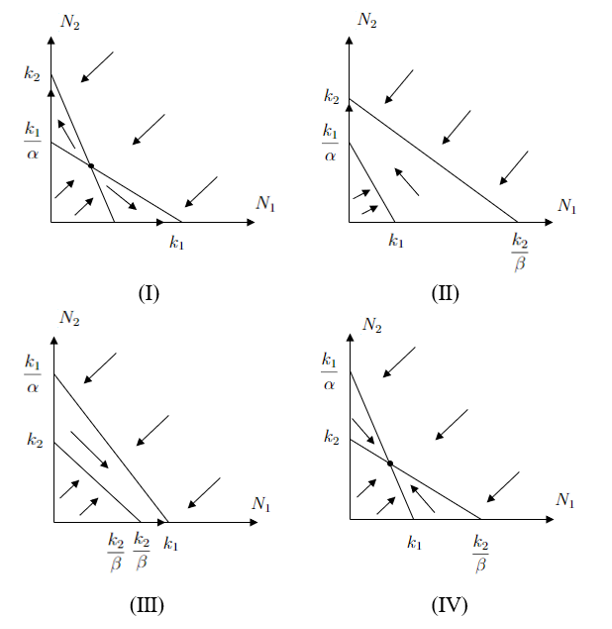
\includegraphics[width=0.55\textwidth]{./code/fig6.png}
        \caption{Four results represented by balance lines}\label{fig6}
    \end{figure}
    
By using the curve representation, we can more intuitively observe the interaction between the two fungi and the different evolution of the system under different inhibition relations.
    \begin{figure}[H]
        \centering
        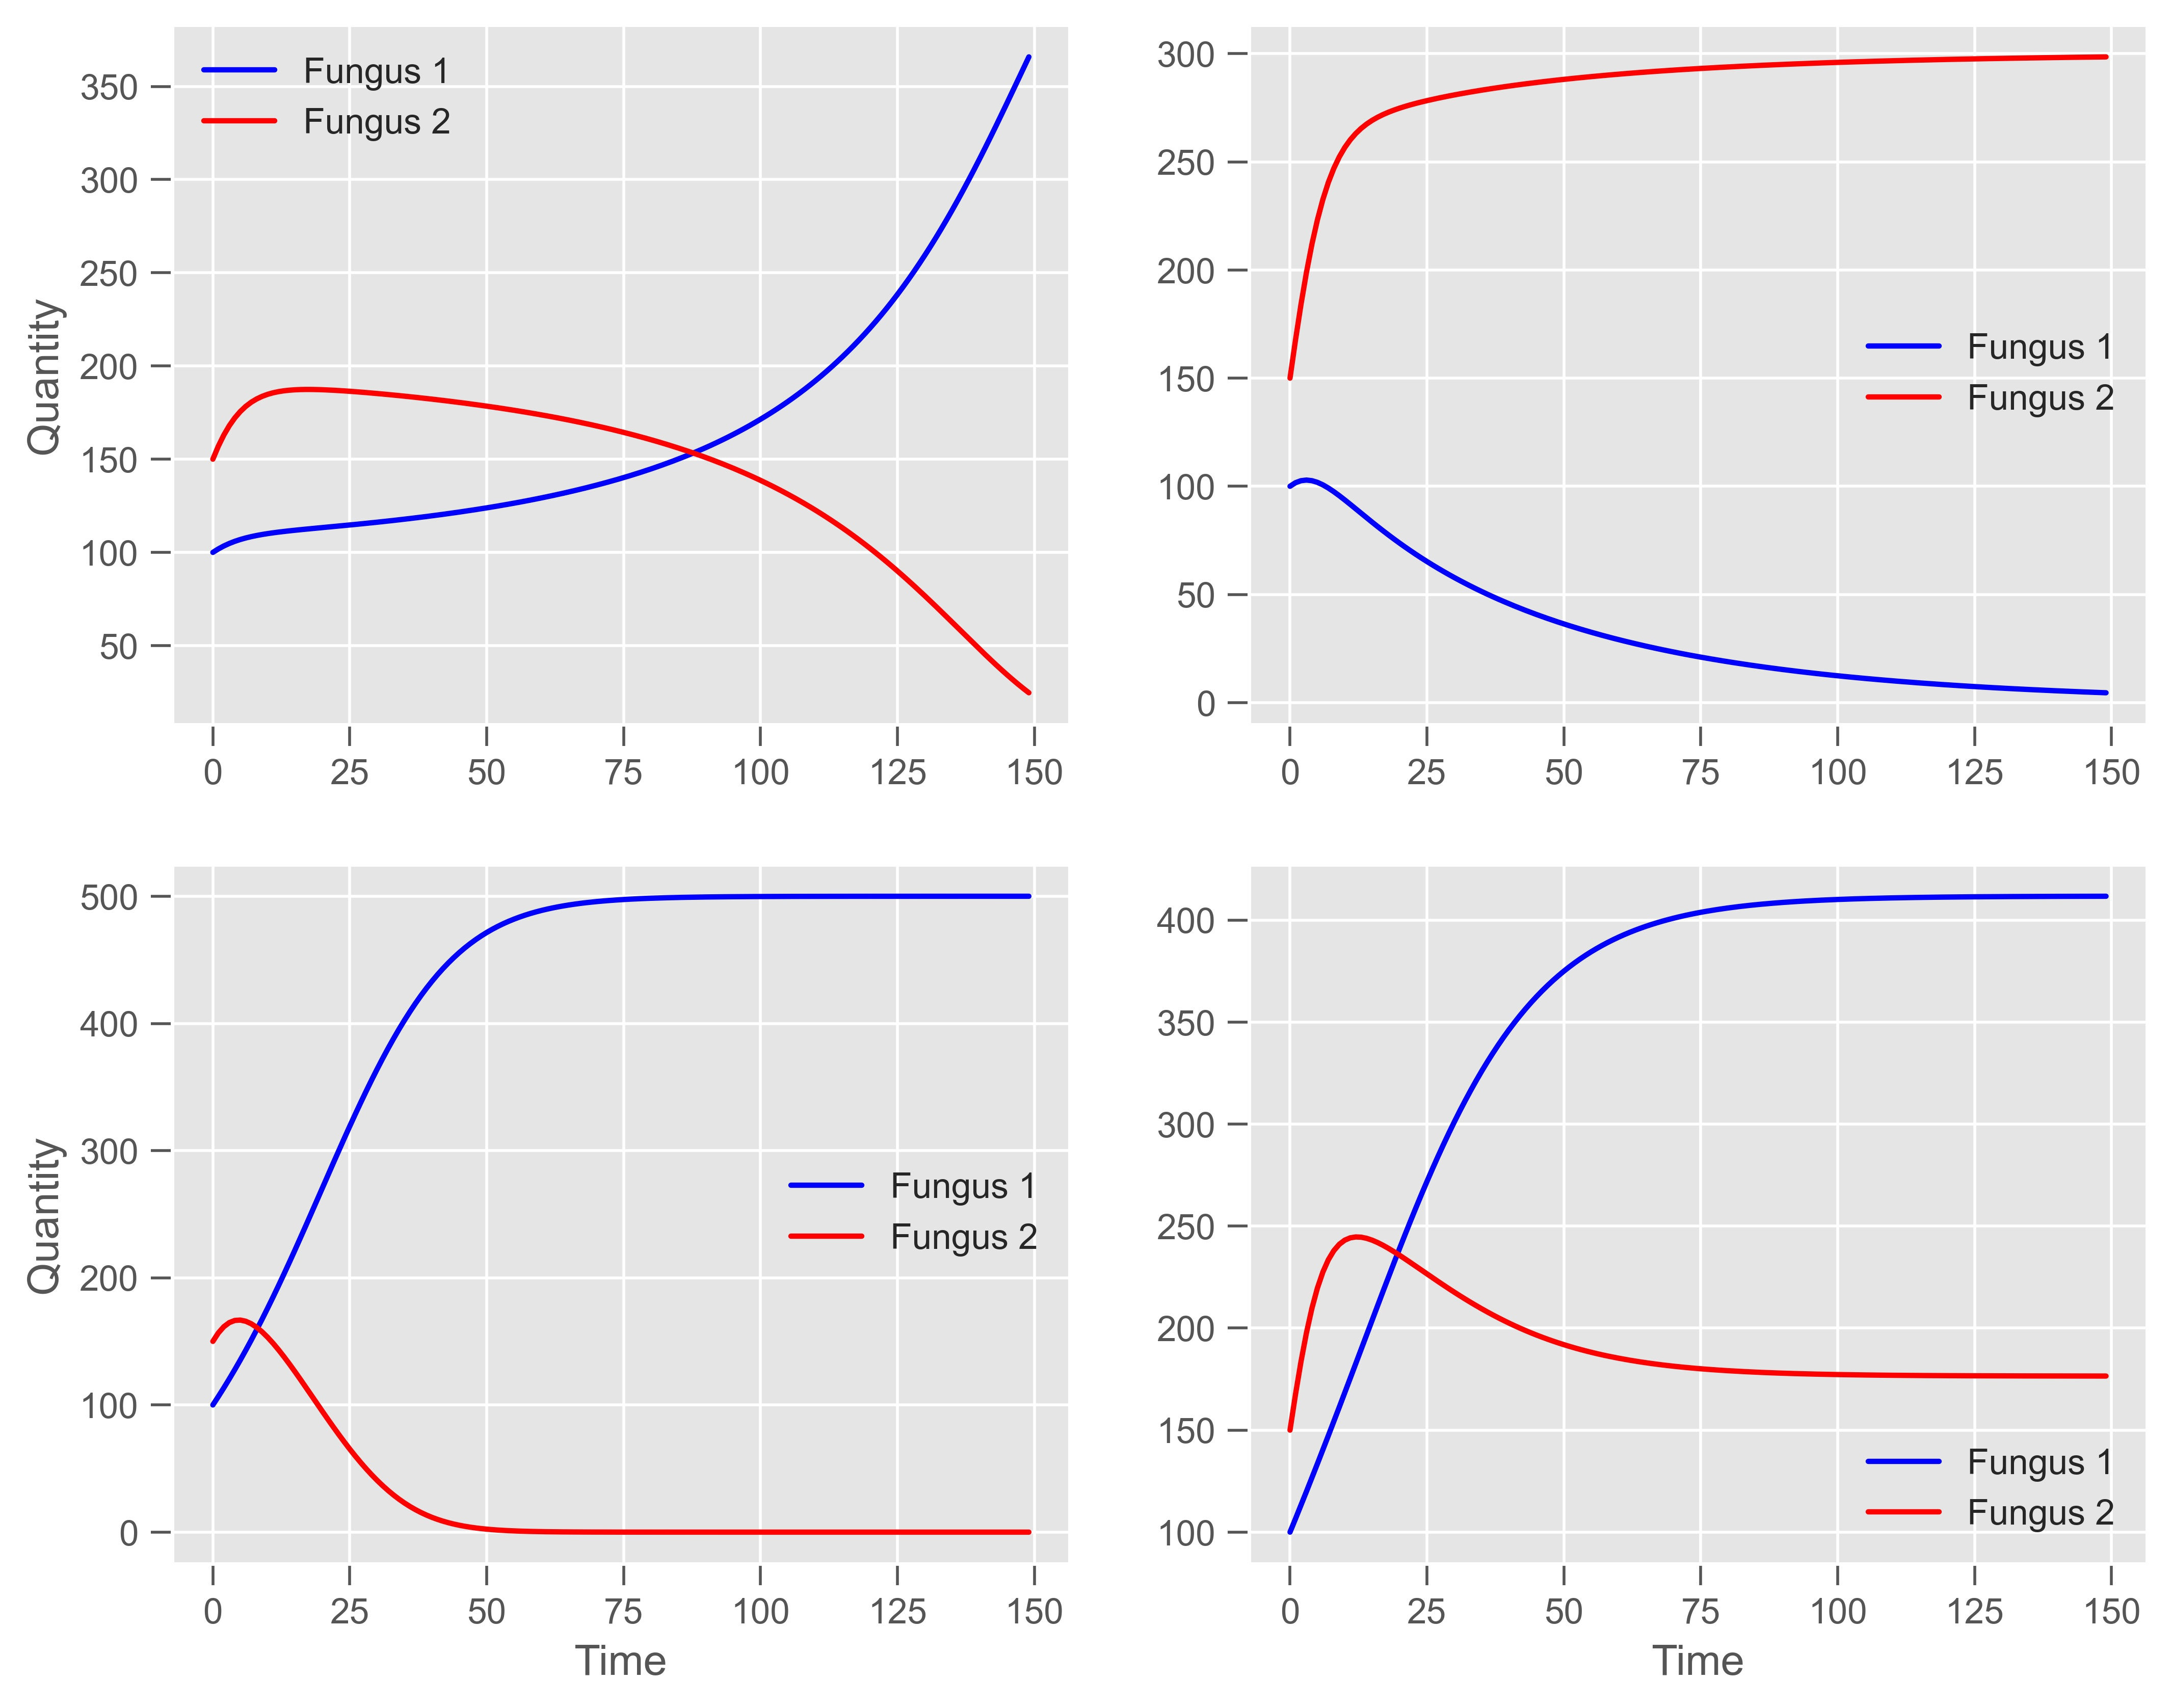
\includegraphics[width=0.6\textwidth]{./code/fig7.jpg}
        \caption{Four results represented by curves}\label{fig7}
    \end{figure}

\subsubsection{Solution of Problem 3}

When the atmospheric environment changes, it will cause changes in the correlation coefficient $k_{1},k_{2},r_{1},r_{2},\alpha,\beta$, which will affect the model and the long-term and short-term trends, resulting in changes in the four situations shown in Figure (\ref{fig6}). Combined with Table (2), it can be seen that situation (\uppercase\expandafter{\romannumeral1}) is most sensitive to the rapid fluctuation of the environment, and the rapid fluctuation determines the direction in which $N_{1},N_{2}$ moves from the equilibrium point and affects which one of Fungus 1 and Fungus 2 is eliminated in the end. That is to say, when $k_{2}>\frac{k_{1}}{\alpha}$ and $k_{1}>\frac{k_{2}}{\beta}$ , the equilibrium state reached is very sensitive to the fluctuation of the atmospheric environment. Situation (\uppercase\expandafter{\romannumeral1}) (\uppercase\expandafter{\romannumeral2})and (\uppercase\expandafter{\romannumeral3}) has a certain ability to adjust the change of $N_{1},N_{2}$. In the short term, it will be affected by the fluctuation, but with the passage of time, this influence will be gradually eliminated.

According to the above analysis, the system may have four results when the two types of fungi exist simultaneously. When there is no inhibition between the two fungi, they will eventually reach a stable coexistence state, and the stable point is $E_{4}(k_{1}-\alpha k_{2},k_{2}-\beta k_{1})$ . When one partner is inhibiting the other, eventually the inhibiting partner will gain an advantage and the other partner will be eliminated. When both sides have an inhibiting effect on the other, the initial condition determines the final winner.
